\section{Linear Regression}
\smallskip \hrule height 2pt \smallskip

\underline{Ordinary Least Squares} \hfill \\

Notation:
\begin{itemize}
	\item \textbf{$x_i$}: an input data point.  \_\_ rows by \_\_ columns. 
	\item \textbf{$y_i$}: a predicted output
	\item \textbf{$\widehat{y_i}$}: a predicted output
	\item \textbf{$\widehat{y}$}: 
	\item \textbf{$w_k$}: weight k
	\item \textbf{$\bm{w}*$}:
	\item \textbf{$f_k(x_i)$}
	\item \textbf{$t_j$}: the output variable that you either have data for or are predicting. 
	\item \textbf{$t(\bm{x})$}: Data.  "Mapping from x to t(x)"
	\item \textbf{$H$}: $H = \{ h_1, \dots, h_K \}$.  Basis functions.  In the simplest case, they can just be the value of an input variable/feature or a constant (for bias).  
\end{itemize}

\underline{Vocab}:
\begin{itemize}
	\item \textbf{basis function}
	\item \textbf{bias} - like the intercept in a linear equation.  The part that doesn't depend on the features. 
	\item \textbf{hyperplane} - a plane, usually with more than 2 dimensions. 
	\item \textbf{input variable} - a.k.a. feature.  % https://en.wikipedia.org/wiki/Dependent_and_independent_variables
		E.g. a column like CEO salary for rows of data corresponding to different companies.
	\item \textbf{response variable} - synonyms: "dependent variable", "regressand", "predicted variable", "measured variable", "explained variable", "experimental variable", "responding variable", "outcome variable", and "output variable".   E.g. a predicted stock price.   
	\item \textbf{regularization} -  introducing additional information in order to solve an ill-posed problem or to prevent overfitting. 
	% https://en.wikipedia.org/wiki/Regularization_(mathematics)
	E.g. applying a penalty for large parameters in the model. 
	\item \textbf{ridge regression} - 
\end{itemize}

\underline{Ordinary Least Squares}: \hfill \\
total error = $\displaystyle \sum_i (y_i-\hat{y_i})^2 = \sum_i(y_i - \sum_k w_k f_k(x_i))^2$ \hfill \\
Under the additional assumption that the errors be normally distributed, OLS is the maximum likelihood estimator. \hfill \\ % https://en.wikipedia.org/wiki/Ordinary_least_squares
?? Use words to describe what subset of regression in general this is.  What is ordinary? What are we limiting?  \hfill \\
 \hfill \\

The regression problem: \hfill \\
Given basis functions $\{ h_1, \dots, h_K \}$  with $h_i(\bf{x}) \in \mathbb{R}$,  \hfill \\
	find coefficients $\bm{w} = \{ w_1, \dots, w_k \}$.  \hfill \\%  
$t(\bm{x}) \approx \widehat{f}(\bm{x}) = \sum_i w_i h_i(\bm{x})$ 

This is called linear regression b/c it is linear in the parameters. 
We can still fit to nonlinear functions by using nonlinear basis functions. 
Minimize the \textbf{residual squared error}: \hfill \\
$ \displaystyle \bm{w}* = \argmin_{\bm{w}}  \sum_j (t(\bm{x}_j) - \sum_i w_i h_i(\bm{x}_j))^2$
\hfill \\  \hfill \\

For fitting a line in 2D space, your basis functions are $\{ h_1(x) = x, h_2(x) = 1 \}$  \hfill \\  \hfill \\

To fit a parabola, your basis functions could be $\{ h_1(x) = x^2, h_2(x)=x, h_3(x)=1 \}$.   \hfill \\
Want a 2D parabola? Use $\{ h_1(x) = x_1^2, h_2(x)=x_2^2, h_3(x)=x_1 x_2, \dots \}$. \hfill \\
Can define any basis functions $h_i(\bm{x})$ for n-dimensional input $\bm{x} = <x_1, \dots, x_n>$
\hfill \\  \hfill \\

\underline{Regression: matrix notation}: \hfill \\
\begin{align*}
	\bm{w}* &= \argmin_w \sum_j(t(\bm{x}_j - \sum_i w_i h_i(\bm{x}_j))^2  \\
	\bm{w}* &= \argmin_w (\bm{Hw} -\bm{t})^T (\bm{Hw} -\bm{t})
\end{align*}
$  (\bm{Hw} -\bm{t})^T (\bm{Hw} -\bm{t})$ is the residual error. 
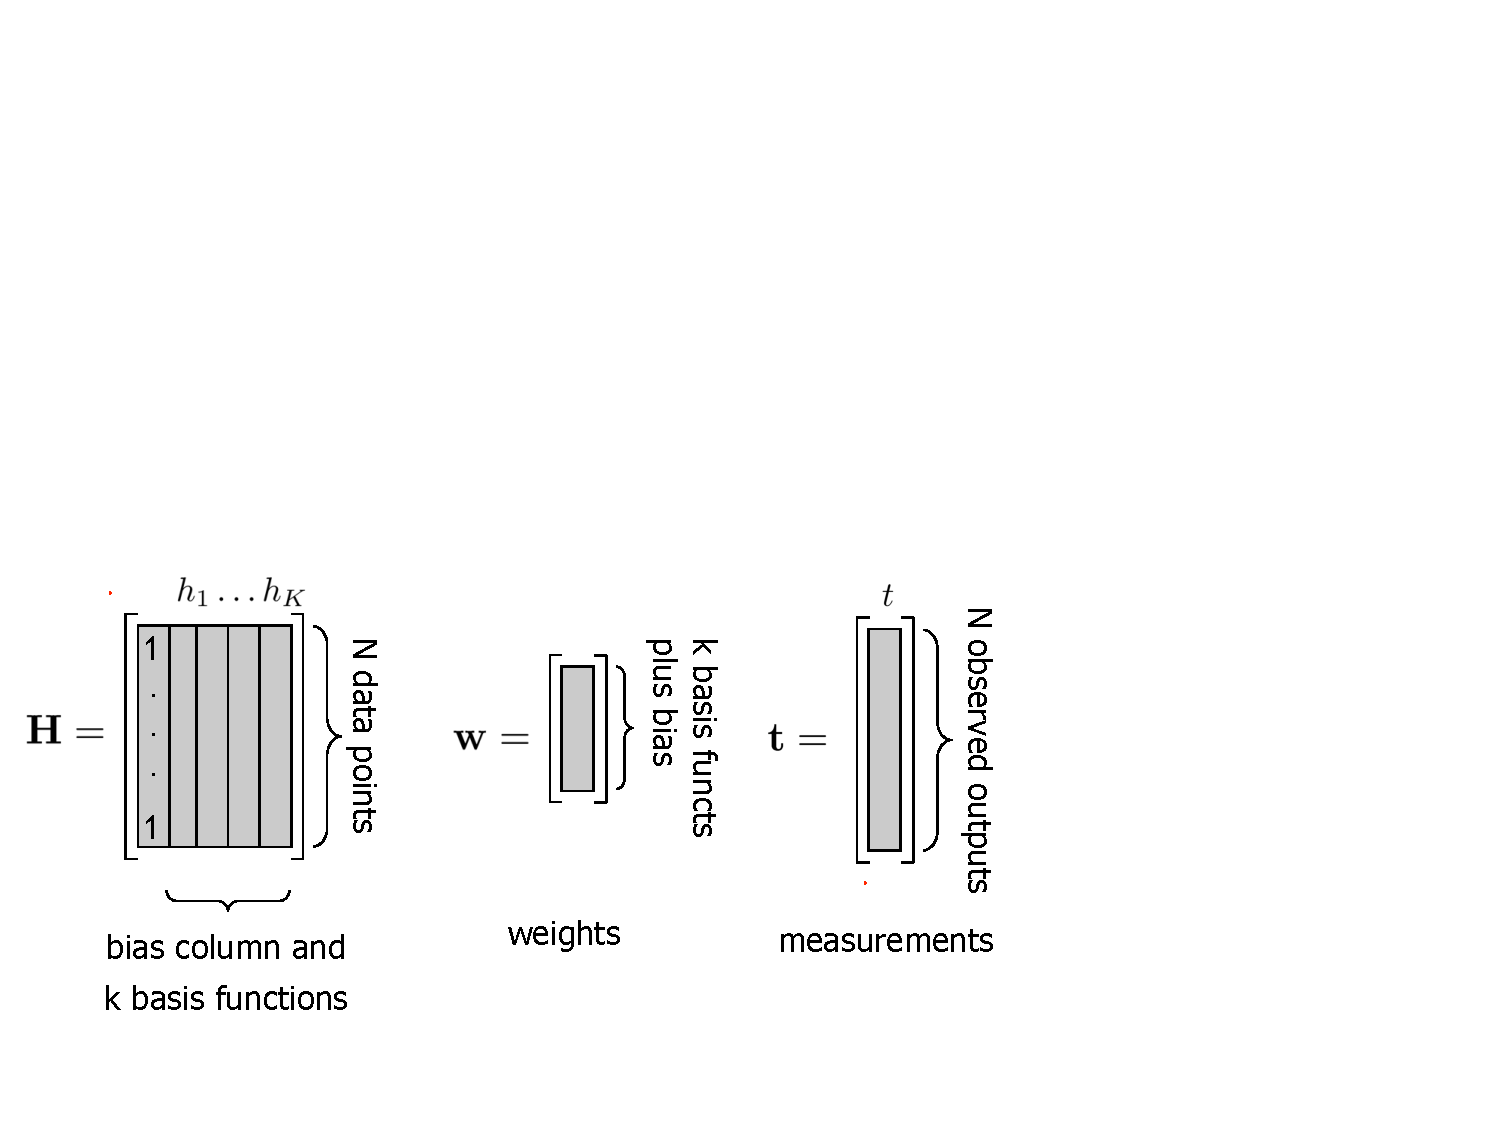
\includegraphics[width=3in]{figures/Least_squares_matricies.pdf}

\underline{Regression: closed form solution}:  % derivation: http://courses.cs.washington.edu/courses/cse446/16wi/Slides/4_LinearRegression.pdf
\begin{align*}
	\bm{w}* = \argmin_w (\bm{Hw} -\bm{t})^T (\bm{Hw} -\bm{t})  & \\
	\bm{F}(\bm{w}) =  \argmin_w (\bm{Hw} -\bm{t})^T (\bm{Hw} -\bm{t}) & \\
	\triangledown_{\bm{w}}\bm{F}(\bm{w}) = 0 \\
	2 \bm{H}^T (\bm{H}\bm{w}-\bm{t}) = 0  & \\
	(\bm{H}^T\bm{H}\bm{w}) - \bm{H}^T\bm{t} = 0 & \\
	\bm{w}* = (\bm{H}^T\bm{H})^{-1}\bm{H}^T\bm{t} &
\end{align*}

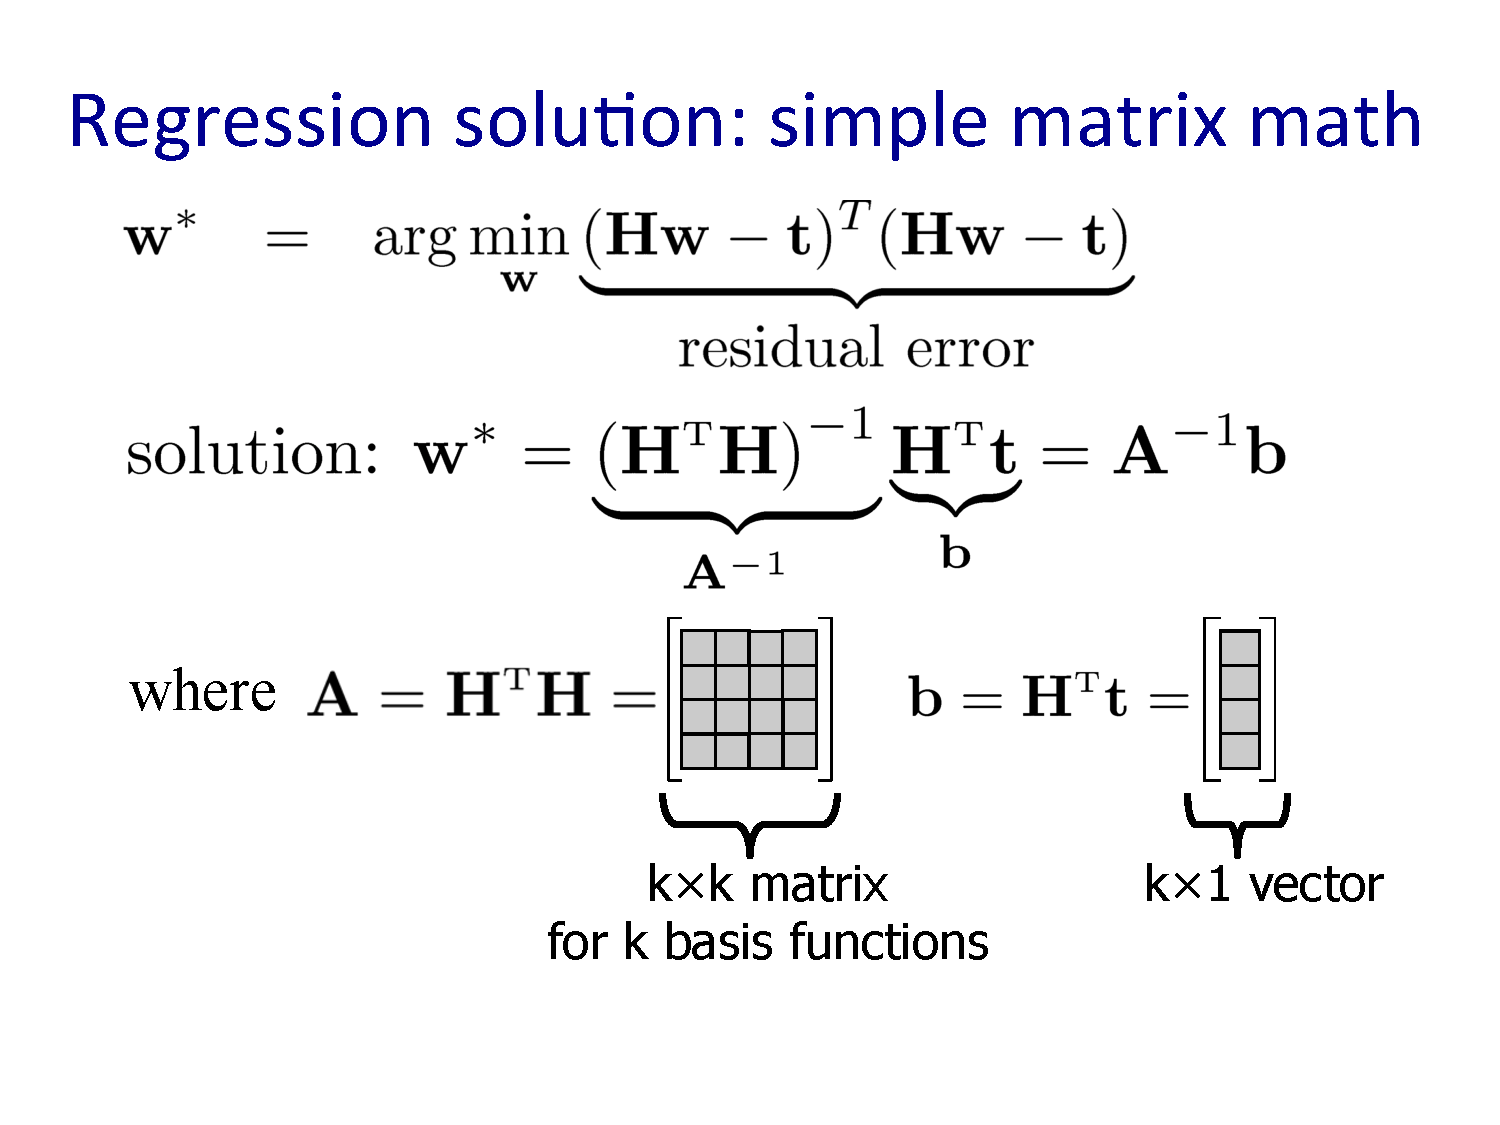
\includegraphics[width=3in]{figures/Regression_matrix_math.pdf}

Linear regression prediction is a linear function plus Gaussian noise:  \hfill \\
$t(\bm{x}) = \sum_i w_i h_i(\bm{x}) + \epsilon $ \hfill \\
We can learn $\bf{w}$ using MLE: 
$P(t | x, w, \sigma) = \frac{1}{\sigma \sqrt{2 \pi}} e^\frac{-[t - \sum_i w_i h_i(x)]^2}{2 \sigma^2}$
Take the log and maximize with respect to w:  (maximizing log-likelihood with respect to w) \hfill \\
$\displaystyle \ln P(D | \bm{w}, \sigma) = \ln(\frac{1}{\sigma \sqrt{2 \pi}})^N \prod_{j=1}^N e^\frac{-[t_j - \sum_i w_i h_i(x_j)]^2}{2 \sigma^2}$ \hfill \\
Now find the w that maximizes this: \hfill \\
$\argmax_w \ln(\frac{1}{\sigma \sqrt{2 \pi}})^N + \sum_{j=1}^N \frac{-[t_j - \sum_i w_i h_i(x_j)]^2}{2 \sigma^2}$ \hfill \\
the first term isn't impacted by $w$ so  \hfill \\
$= \argmax_w  \sum_{j=1}^N \frac{-[t_j - \sum_i w_i h_i(x_j)]^2}{2 \sigma^2}$ \hfill \\
switch to $\argmin_w$ when we divide by -1.  The numerator is constant.:  \hfill \\
$= \argmin_w  [t_j - \sum_i w_i h_i(x_j)]^2 $ \hfill \\

\textbf{Least-squares Linear Regression is MLE for Gaussians!!!}  \hfill \\ \hfill \\

\underline{Regularization in Linear Regression}  \hfill \\


 